%%%%%%%%%%%%%%%%%%%%%%%%%%%%%%%%%%%%%%%%%%%%%%%%%%%%%%%%%%%%%%%%%%%%%%%%%%%%%%%%
%2345678901234567890123456789012345678901234567890123456789012345678901234567890
%        1         2         3         4         5         6         7         8

%\documentclass[letterpaper, 10 pt, conference]{ieeeconf}  % Comment this line out
                                                          % if you need a4paper
                                                         
\documentclass[a4paper, 10pt, conference]{ieeeconf}      % Use this line for a4
                                                          % paper

\IEEEoverridecommandlockouts                              % This command is only
                                                          % needed if you want to
                                                          % use the \thanks command
\overrideIEEEmargins
% See the \addtolength command later in the file to balance the column lengths
% on the last page of the document



% The following packages can be found on http:\\www.ctan.org
\usepackage{graphics} % for pdf, bitmapped graphics files
\usepackage{epsfig} % for postscript graphics files
\usepackage{mathptmx} % assumes new font selection scheme installed
\usepackage{times} % assumes new font selection scheme installed
\usepackage{amsmath} % assumes amsmath package installed
\usepackage{amssymb}  % assumes amsmath package installed

\usepackage{multirow}

\usepackage{graphicx}
\usepackage{float}
\usepackage{fancyhdr}

\usepackage[T1]{fontenc}
\usepackage{textcomp}
\usepackage{gensymb}

\usepackage[utf8x]{inputenc}

\title{\LARGE \bf
Event Extraction From Radio News Bulletins For Linked Data
}
%\author{K. E. van Putten}

\author{ \parbox{3 in}{\centering K. E. van Putten\\
%         \thanks{*Use the $\backslash$thanks command to put information here}\\
         Bcs Computer Science\\
         1083 HP Amsterdam, The Netherlands\\
         {\tt\small ke.vanputten@gmail.com}}
         \hspace*{ 0.5 in}
}

\begin{document}


\date{\today}
\maketitle
%\thispagestyle{empty}
%\pagestyle{empty}
\pagestyle{plain}


%%%%%%%%%%%%%%%%%%%%%%%%%%%%%%%%%%%%%%%%%%%%%%%%%%%%%%%%%%%%%%%%%%%%%%%%%%%%%%%%
\begin{abstract}

Abstract

\end{abstract}


%%%%%%%%%%%%%%%%%%%%%%%%%%%%%%%%%%%%%%%%%%%%%%%%%%%%%%%%%%%%%%%%%%%%%%%%%%%%%%%%

\section{Introduction}
The internet contains a seemingly unlimited sea of information, and navigating this see can be daunting. Online search has become an increasingly important application on the web, and many users who browse the internet today make use of traditional keyword-based search engines such as Google or Bing. While these search engines are excellent for retrieving targeted information they do require the user to have a well defined information need which can be captured in carefully designed search queries. Exploratory search on the other hand provide information retrieval to users with an unclear information need. Exploratory search systems offer support for browsing strategies through carefully designed interfaced which support interactive forms of search \cite{marchionini2006exploratory}.

\subsection{DIVE+}

DIVE+ is an event-centric linked data browser which aims to provide exploratory search within an integrated heterogeneous dataset of historical media objects \cite{de2015dive}. It was designed to support digital humanities scholars in their online exploration and research. The DIVE+ browser facilitates exploration and learning through an intuitive and interactive interface which allows the end user to browse media objects from four different heritage institutions, namely the Netherlands Institute for Sounds and Vision (NISV), the Dutch National Library (KB), the Amsterdam Museum (AM), and the Tropenmuseum (KIT).\cite{ineldive+}  

The media objects in the dataset are structured and interlinked using Linked Data. All objects are enriched with meta-data which include descriptive text, related entities such as actors and places, and events. Van den Akker et al. \cite{van2011digital} describe events as a relationship between an object and an event that has historical meaning. These relationships are utilized to create the links between the media objects. This way when a user searched for an object, they will also be presented with other media objects which are related to the object they are currently viewing. Objects may be related because they describe the same event, they are related to events that involve the same place, actors or type, or because objects are used or function in a shared event. By presenting the user with related objects, the user might stumble upon unexpected objects or discover new research topics. 

\subsection{Problem Statement}

In order to structure and link the media objects in the dataset, the events and related entities first need to be identified. Because of the vast size of the dataset of DIVE+ it is not viable to annotate these entities and events manually and an automated ways of Information Extraction (IE) would be preferred. Named Entity Recognition (NER) is a subtask of IE which aims to identify Named Entities (NE) and classify them into predefined categories. For the enrichment of the DIVE+ data, several NER tools such as NERD, TextRazor, THD, DBpediaSpotlight, Lupedia and SemiTags are used to extract NE's of type persons, locations, and concepts\cite{de2015dive}.

While NE extractors typically show good results\cite{gangemi2013comparison} they do not all feature event detection, and when they do they often struggle to extract events correctly and link events to their role fillers (participants, locations and time concepts). Event extraction proved to be particularly difficult for media objects from the KB library, which are Dutch radio news bulletins from the period 1937-1984. Better methods of event extraction are needed in order to properly integrate these objects in the linked data structure and to create links between related radio bulletins, and between radio bulletins and objects from the other cultural heritage library sources.

\subsection{Research Question}
In line with the problem statement, we have formed the following research question: \textit{"Can we find a more effective way to extract events from the KB radio news bulletins to improve linkage within the DIVE+ system?"}

Because of the experienced difficulties with event extraction, the radio news bulletins from KB currently have all have one event in their meta-data. These events are actually a best guess rather than proper extracted events. The first 100 characters from each bulletin's content were taken as the bulletin's event with the underlying thought that often times the most important topics are mentioned that the beginning of a text. Our aim it to find a better approach to extracting events from the KB radio news bulletins rather than extracting the first 100 characters.

\section{Related Work}
Event extraction is used in may applications and there are various methods of extracting events. In this section we will briefly discuss related research and studies on the topic of event extraction.

\subsection{Methods of Event Extraction}\label{related work methods}
There exist various methods of event extraction. In their paper, Hogenboom et al.\cite{hogenboom2011overview} make a distinction between three types of approaches of event extraction, namely knowledge-driven, data-driven and a hybrid form of event extraction that combines knowledge-driven and data-driven event extraction methods, and analyze and compare several approaches of event extraction in these categories. 

Hogenboom et al. define data-driven approaches as a quantitative methods to discover statistical relations. For example through word frequency counting, clustering or ranking by means of the Term Frequency - Inverse Document Frequency (TF-IDF) metric. Hogenboom et al. argue that the drawbacks of data-driven event extraction approaches are that they discover relations in texts without considering semantics. Furthermore, data-driven approaches require large amounts of data in order to get statistically significant results.

Knowledge-driven approaches on the other hand require significantly less data, but they do require expert knowledge of the texts. Knowledge-driven methods mine information from corpora by searching for defined linguistic patterns (either lexico-syntactic patterns or lexico-semantic patterns) in texts. Hogenboom et al. argue that the advantage of knowledge-based event extraction methods is that these methods require less training data and the returned results from pattern-based approaches are often easier to interpret and more traceable. However, knowledge-based extraction also has it's downsides. Lexical knowledge, and often also prior domain knowledge, is required in order to define powerful expressions that retrieve the desired information. Furthermore, it can be difficult to scale up pattern based approaches to cover more situations because patterns are often hand-tuned. Acquiring and maintaining a large set of pattern based rules is costly, systems are often build for a specific type of texts and portability is poor when the system is ported to other domains or languages, and lastly adding new rules that aim to improve in a local area may result in poorer performance globally (also known as the 'seesaw phenomena')\cite{su1996overviewCBSO}.

Hogenboom et al. describe hybrid approaches as event extraction methods which equally combine knowledge-driven and data-driven approaches. Since both data-driven and knowledge-driven approaches have their disadvantages, they may complement each other and when used together such that the two approaches complement each others weak points they might yield the best results.

%They conclude that knowledge-driven event extraction methods, which extract knowledge through representation and exploitation of expert knowledge, usually by means of pattern based approaches, require the least amount of data. For knowledge-driven event extraction experiments can be performed on as little as a few hundred documents or sentences, but for this method a high amount of expert and domain knowledge is required. Data-driven approaches, which rely on quantitative methods to discover relations such as through the usage of statistics, machine learning or linear algebra, require the most amount of data in order to develop models that approximate linguistic phenomena but little expert and domain knowledge is required for these approaches.  Hybrid approaches require fewer documents than data-driven approaches to report results, but can still require up to a couple thousand documents. 

Atefeh and Khreich\cite{atefeh2015survey} classify event detection methods into document-pivot and feature-pivot techniques. 

Document-pivot techniques are event detection techniques that detect events by clustering documents based on their textual similarity. This type of event detection has been addressed in the Topic Detection and Tracking (TDT) research program which aims to organize and structure broadcast textual news objects from a multitude of media sources by detecting events (in TDT parlance called a \textit{topic}) and linking stories that discuss the same event\cite{allan1998topic}. In TDT, event detection has been broadly divided into two categories: retrospective event detection (RED)\cite{yang1998studyofretrospective} and new event detection (NED)\cite{allan1998line}. RED focuses on discovering previously unidentified events in historical news data collections, whereas NED (also known as first-story detection or novelty detection) aims to discover new events from live streams of news documents. Clustering based algorithms have been mainly utilized for both categories of event detection\cite{atefeh2015survey}. Atefeh and Khreich conclude that hierarchical clustering approaches have been widely employed for RED because RED involves iterative clustering algorithms that organize all documents from a collection into event clusters, while greedy clustering algorithms are more commonly used for NED tasks in order to cluster documents with preexisting clusters or create new clusters when the arriving documents describe new events. They conclude that document-pivot techniques assume that all input data contain some new or old events, which means that these techniques are not really suitable when the input contains irrelevant data.

Feature-pivot techniques detect events by bursty   

Naughton et al.\cite{naughton2006event} implemented and compared two data-driven approaches of event extraction from news articles by means of sentence clustering. For the first described method, each sentence in the news article was reduced to stemmed terms and similar sentences describing the same event were clustered together. The second described method is a sequence-bases solution aimed to exploit article structure by giving preference to clustering sentences which are located near each other in the text. Naughton et al. reason that adjacent sentences are more likely to refer to the same event. Lastly, they introduced a variation to the two clustering algorithms by adopting a Machine Learning-based approach to filter sentences which did not describe any events from the text before the clustering stage.

%%%%%%%%%%%%%%%%%%%%%%%%%%%%%%%%%%%%%%%%%%%%%%%%%%%%%%%%%%%%%%%%%%%%%%%%%%%%%%%%

\begin{figure*}[!h]
  \centering
  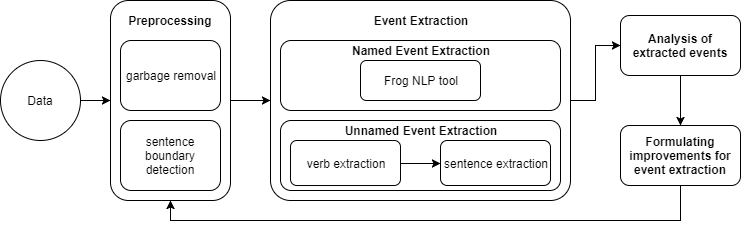
\includegraphics[width= \textwidth]{Temp_Pipeline}
  \caption{Pipeline of the research methodology.}
  \label{pipeline}
\end{figure*}

\section{Methodology}
The following sections will describe the stages of our research of finding a better method to extract events from the radio bulletins. We start with our data selection and a data description in section \ref{data}. Section \ref{preprocessing} will discuss the steps taken during the preprocessing of the data. Section \ref{extraction} will describe the extraction of events from the radio bulletins and in section \ref{analysis} we will analyze the results from the event extraction step. Lastly, section \ref{improving} will elaborate on the ways in which we attempted to improve the event extraction process.

%%%%%%%%%%%%%%%%%%%%%%%%%%%%%%%%%%%%%%%%%%%%%%%%%%%%%%%%%%%%%%%%%%%%%%%%%%%%%%%%

\subsection{Data}\label{data}
The Dutch National Library provides access to a large number of historical datasets. DIVE+ uses the KB ANP Radio News Bulletins dataset\footnote{http://www.delpher.nl/nl/radiobulletins/}, which contains digitized typoscripts from the period 1937-1984. These typoscripts are news scripts which were read during news broadcasts on the radio. All the typoscripts are Dutch texts. From this data we selected a subset of 215 news bulletins which are all dating from April 1939. We selected data from the same time period so that the typoscripts will mention related historical events which will allow us to establish new links between these bulletins if the event extraction works successfully.

The radio news bulletins are typoscript documents which are enriched with metadata. The metadata consists of the following items:
\begin{itemize}
\item Descriptive text content. The descriptive text content stores a description of the media object. In the case of the ANP bulletins, the descriptive text contains the text extracted from the original typoscript documents. The documents were scanned and put through optical character recognition (OCR) software to convert the images of the scanned documents to machine-encoded text. 

\item The date related to the media object. For the news bulletins the date is the day on which the bulletin was read on the radio.

\item Named Entities (NEs). Entities related to the media object are identified, extracted and stored in the metadata. The NEs of the ANP radio news bulletins are classified into three categories; actors, places, and other related concepts. Actors can be persons or organisations such as \textit{Minister Slotemaker de Bruine}, \textit{Padvindersbond}, or \textit{Nederlandsche Jeugdherberg Centrale}. Places are any entities that indicate a location, such as countries, cities, or buildings. Lastly, other related concepts are entities which are related to the media object but are not actors or places. Examples of other related concepts are \textit{Holland-Amerika-lijn}, \textit{Barakkenkamp}, and \textit{Foreign Office}. Table \ref{NE count} depicts the number of NEs in the selected subset of 215 bulletins. 

\begin{table} [b]
  \begin{center}
    \begin{tabular}{l|r}
    Named Entity type & Count\\
    \hline
    Actors & 1296\\
    Places & 526\\
    Other related concepts & 526
    \end{tabular}
  \end{center}
  \caption{Number of Named Entities in the selected subset of the KB data.}
  \label{NE count}
\end{table}

\item Events. These form the core building blocks on which the linked data structure is formed. The metadata of the radio bulletins contain precisely one event. Since no effective way of extracting events from the KB bulletins had yet been found, a 'best guess' was made by extracting the first 100 characters from the descriptive content. Reasoning for this was that the most important events are often mentioned at the start of a text. Thus, by extracting the first part of the text it was hoped that these strings would contain the main event of the news bulletin.
\end{itemize}

%example of data%
Figure \ref{bulletin} in the Appendix shows and example of an ANP radio news bulletin in the DIVE+ demonstrator. The right shows the scanned typoscript document. The left shows the descriptive text, which is the content of the document which was extracted by OCR software. The bottom of the image shows the number of extracted NEs. This particular bulletin has one event and seven NEs in the metadata.

%problems with data%
This example bulletin also shows several issues in the data that are problematic for the event extraction. 

Firstly, we can see that the OCR did not extract the text content from the document flawlessly. Words that were crossed out in the typoscript resulted in garbage strings such as \textit{v\char`\^HMMHHMMM|MMHM$))$} in the OCR output. We also see many instances were the OCR software misidentified characters, resulting in spelling errors such as \textit{$Zuldwearenwlnd$} instead of \textit{Zuidwestenwind}. Not only do these errors in the descriptive content make the text difficult to read for users, but we also observed during the event extraction process that Natural Language Processing (NLP) tool struggle with their task when the input text contains errors. 

Secondly, we see that the NEs in the metadata are not always correct or complete. The NEs that were identified in the bulletin in figure \ref{bulletin} are: \textit{Arrondiaaeaantareoht} (place), \textit{Geroohtahof} (place), \textit{Woetkant} (place), \textit{Staatsoourant} (actor), \textit{W. C. CALKOEN} (actor), \textit{W. E. J. BOLLEE} (actor), and \textit{Zuldweatenwlnd} (actor). We see that \textit{Staatsoourant} and \textit{Zuldweatenwlnd} were incorrectly classified as actors and \textit{Arrondiaaeaantareoht} (arrondissementsrechtbank) was incorrectly classified as a place. On the other hand, \textit{DEN HAAG} and \textit{CULEHBORG} were not extracted as NE's while they are places. 

%%%%%%%%%%%%%%%%%%%%%%%%%%%%%%%%%%%%%%%%%%%%%%%%%%%%%%%%%%%%%%%%%%%%%%%%%%%%%%%%

\subsection{Preprocessing}\label{preprocessing}
As described in the previous section, \ref{data}, the descriptive content of the bulletins contain errors caused by the OCR extraction. Because we attempt to extract historical events related to the objects from the descriptive content, we first execute data preprocessing steps to prepare the data for the event extraction step. We  perform garbage removal from the texts which will be described in section \ref{garbage removal}. The other preprocessing step, which is sentence boundary detection, will be discussed in section \ref{sbd}.

\subsubsection{Garbage Removal}\label{garbage removal}~\\
In order to make the text content of the bulletins more readable, for both person and machine, we try to remove garbage strings caused by handwritten notes and blacked out text on the scanned documents. To do this we adopt a pattern-based approach. We implemented pattern-based rules for recognizing garbage strings in texts which were formulated by Taghva et al.\cite{taghva2001automatic}. We implemented and made adjustment to these rules to achieve better garbage removal from the KB bulletin texts specifically.

We split the OCR text of each bulletin into \textit{strings}, which we define as a stream of characters separated by whitespace. \textit{Garbage strings} are defined by the rules listed below. When a string is identified as a garbage string, it is automatically removed from the text. The rules, including examples of garbage strings which were found and removed from the data:
\begin{itemize}
\item (L) If a string is garbage if it is longer than 30 characters:

\textit{$nahaaxaKnKBBnBaBnxmBnRaxmga\%BH6anih\&$} 

\textit{$3a\char`\^*3§!B3ta\char`\^\ast swN\ast9\ast33EaSBbS\$P2ri9BP$}

\item (A) If the number of alphanumeric characters in a string is less than \%50 of the total number of characters of the string, then the string is garbage:

\textit{$\ast\ast\ast S\ddot{\mathrm{E}}P'.$}

\textit{$-P=\ast\char`\^,$}

\textit{$\char`\^t**-********b\ast\hat{\mathrm{e}}$}

\item (R) If a string contains four identical characters in a row, it is garbage:

\textit{$ixxxxxtgHxaHRn$}

\textit{$HHHHSRHEHHMHH$}

\textit{$nnnn\&$}

\item (V) If a string only contains alphanumeric characters, we count the number of consonants and vowels. If the number of consonants is less than 10\% of the number of vowels, or the number of vowels is less than 10\% of the number of consonants, then the string is garbage:

\textit{$mmimmmnnsmfl$}

\textit{$eeIe$}

\textit{$n$}

\item (P) If the string contains two or more distinct punctuations, ignoring the first and last character of the string, then it is removed as garbage. For example, the string \textit{12,3.} is not removed because we ignore the last character of the string, but \textit{12,3/.} is.

\textit{$\degree S\char`\^\ddot{\mathrm{e}}2\%Bn'ene$}

\textit{$3T\ast-\char`\^3$}

\textit{$Vo\backslash o::$}

\item (C) If the first and last characters of the string are lowercase letters, and the string contains an uppercase letter anywhere between, and the character directly before the uppercase letter is an alphanumeric character, then the string is removed. This means that \textit{aaAaa} gets removed, but \textit{park-Eindhoven} is not.

\textit{$anafBBsi$}

\textit{$a3Hb$}

\textit{$zntaH\#saxnihxhsh$}

\end{itemize}

Rules (A), (R), (V) and (P) were directly adopted from the paper by Taghva et al.\cite{taghva2001automatic}. Rules (L) and (C) were slightly altered from the similarly labeled rules described by Taghva et al. for more accurate garbage removal from the bulletin texts. We changed rule (L) from a 40 character to a 30 character threshold, because we observed that the OCR extracted texts barely contained any strings longer than 40 characters, while the majority of the strings between 30 and 40 characters were garbage. We changed rule (C) to not remove stings when the character prior to the uppercase letter is punctuation. This was done to prevent strings such as \textit{britsch-Italiaansohe} from getting removed.

Overall 2,574 strings were removed from the data. Table \ref{garbage removed per rule} shows how many strings were removed from the texts per defined rule.

%seesaw effect%

\begin{table}
  \begin{center}
    \begin{tabular}{c|r}
    Rule & Strings removed\\
    \hline
    (L) & 15\\
    (A) & 660\\
    (R) & 61\\
    (V) & 1,357\\
    (P) & 244\\
    (C) & 237\\
    \end{tabular}
  \end{center}
  \caption{The number of garbage strings identified and removed per rule}
  \label{garbage removed per rule}
\end{table}

\subsubsection{Sentence Boundary Detection}\label{sbd}~\\
During the event extraction step, which will be discussed in section \ref{extraction}, we will extract full sentences from the text which contain events. In order to do so, it is necessary to know where each sentence in the text begin and end. This is why sentence boundary detection is a required step in preprocessing.

Texts that are written for radio, especially news bulletins, are written with clear and neutral language so that the message can be clearly understood by the listening audience\cite{pelgrims2005journalistieke}. Since the data we work with comes from a reliable press agency, we assume that the texts adhere to this style of writing and won't contain expressive language such as rhetoric questions or sentences ending with exclamation points. We assume that all sentences in the data end with a period, and thus that we can determine where a sentence ends by looking at the punctuation.

We discovered that in some of the bulletins the newscaster had put markings at the end of sentences to increase readability. As a result the OCR software would recognize these marks as special characters, most often an asterisk or plus symbol. This is problematic because occasionally the marks would overlap with the punctuation of the text, which meant that the OCR software would recognize and output a special character instead of a period. We therefore implemented another cleanup step to correct the mistakes made by the OCR tool. We scan the descriptive texts for the following four character sequences:

\begin{itemize}
\item $[alphanumeric char][*][uppercase letter]$
\item $[alphanumeric char][*][whitespace][uppercase letter]$
\item $[alphanumeric char][+][uppercase letter]$
\item $[alphanumeric char][+][whitespace][uppercase letter]$
\end{itemize}
When we encounter one of the four sequences in the texts, we replace the asterisk or plus by a period. 

We now split the texts into sentences using the period mark as the delimiter. But periods also occur in abbreviations and initials such as \textit{"den heer F. I. J. W. SCHLOSSER"}. We therefore check that a period is not part of the character sequence $[whitespace][uppercase letter][.]$. When an encountered period appears in such a sequence, the period is not marked as the end of the sentence.

%%%%%%%%%%%%%%%%%%%%%%%%%%%%%%%%%%%%%%%%%%%%%%%%%%%%%%%%%%%%%%%%%%%%%%%%%%%%%%%%

\subsection{Event Extraction}\label{extraction}
In this section, the details of the event extraction will be presented. We distinguish two types of events: \textit{named events} and \textit{unnamed events}. 

Named events are events which have a name. Examples of named events are \textit{Olymische Spelen}, \textit{Tweede Wereldoorlog} and \textit{demonstratie}. We extract these events from the bulletins with the Natural Language Processing (NLP) tool Frog \footnote{https://languagemachines.github.io/frog/}, which will be discussed in section \ref{named}. 

Unnamed events are events which are not labeled with a named. For example, the sentence \textit{"Een aantal hooge functionarissen uit Spaansch Marokko is in RABAT aangekomen."} describes the event of senior officials from Spanish Morocco arriving in Rabat. We take a pattern-based approach to extract unnamed events from the texts, which will be described in section \ref{unnamed}. 

\subsubsection{Named Event Extraction}\label{named}~\\
To extract named events from the bulletins, we used the NLP system Frog. Frog is modular morpho-syntactic tagger, analyzer and parser for Dutch texts\cite{bosch2007Frog}. It uses Part-of-Speech memory-based tagging for NE recognition and information extraction\cite{daelemans2010mbt}. When Frog recognizes a token in the text as a NE, it assigns it a named entity type identifying person, organization, location, product, event and miscellaneous. 

To extract named events from the bulletins, we fed the preprocessed texts to Frog and extracted the tokens which had been identified as NE's of type event from the output produced by Frog. Frog extracted a total of 57 entities which were classified as events from the data.

\subsubsection{Unnamed Event Extraction}\label{unnamed}~\\
As described earlier, unnamed events are not labeled with a name and are described by sentences such as \textit{"Een aantal hooge functionarissen uit Spaansch Marokko is in RABAT aangekomen"} or \textit{"Een groot deel van de Amerikaansche vloot is vanochtend uit VIRGINIE vertrokken"}. This means that unnamed events can not be detected in texts with typical NER tools. 

The extraction of historic events from a news data collection is a retrospective event detection (RED) task. As mentioned in section \ref{related work methods}, a data-driven approach using clustering algorithms is often used for RED tasks. However, data-driven methods require a large set of training data. The dataset we work with is neither large enough, nor do we possess the correct annotations of all the events in the text to effectively train, validate, and test a clustering algorithm. We therefor attempt to extract unnamed events from the bulletins using a knowledge-driven approach which exploits the NE's which have already been identified and are present in the metadata.

The metadata of the bulletins already contains one event per bulletin. These events are a guess at extracting an actual event. The first 100 characters of the descriptive content was taken as the main event of the bulletin. The underlying thought of this method is that the most important event or information is usually found at the beginning of a text. By taking the first 100 characters is was hoped that the extracted strings would at least contain the main event of the news report. However, many of the bulletins start with header information such as the date, radio channel and the news agency that produced the news item, and thus many of the events in the metadata do not actually mention events. We take the reasoning of this approach as our starting point and use the events present in the metadata as our baseline upon which we will improve.

When the text from the documents was extracted by OCR, the formatting of the text such as paragraphs and indentations was lost. This means that we cannot look at the formatting of the text to determine what part of the text is the header and were in the text the actual news reporting starts. To skip past the header, we attempt to extract the main event by identifying the first \textit{eventful sentence}. We define an eventful sentence as a sentence that contains one or more unnamed events.

A simple way to describe unnamed events is as \textit{someone, doing something, somewhere}. Thus, unnamed events can be recognized by pairs of a related actor, action and location. The extracted NE's in the metadata of the bulletins are classified into three types: actors, places and other concepts. This means that we already have knowledge of actors and locations which could be related to an action. We identify actions by means of verb extraction. 

To extract verbs, we used the NLP tool TreeTagger\footnote{http://www.cis.uni-muenchen.de/~schmid/tools/TreeTagger/}. TreeTagger performs probabilistic part-of-speech (POS) tagging using decision trees\cite{schmid2013treetagger} and offers parameter files for a large number of languages including Dutch. Java code was written to tokenize the descriptive texts of the bulletins. Next, the tokenized texts were fed as input to TreeTagger. The tokens which were tagged as verbs were extracted from TreeTaggers output, and their location in the text was determined. Lastly, the tokens were added to the metadata of the bulletins, including their start and end offset and POS tag.

The next step in the extraction process is the sentence extraction. Because we cannot tell precisely which NE's participate in an event or which NE's and verbs are related, we instead extract a sentence which is likely to mention an unnamed event. We assume that the presence of actors, places and verbs in a sentence indicate that the sentence is eventful. By extracting the first eventful sentence in the text we hope to extract the sentence which mentions the main event reported in the text. However, not all unnamed event necessarily involve both an actor and a place. For example, the sentence \textit{"Hij zal woensdag naar Frankrijk terugkeeren"} mentions the event of someone returning to France. It has the action of returning and the location of where the actor is returning to, but the actor itself is not named in the sentence. Instead, \textit{Hij} refers to the actor who is mentioned in an earlier sentence. A second example, the text snippet \textit{"...hebben weer dan driehonderdduizend mijnwerkers vandaag het werk neergelegd"} metions the event of miners laying down work, but there is no associated location in the sentence.

Because not all events might be associated to both an actor and place, we introduce a tiered method of sentence extraction. To extract the first eventful sentence from the text, we identify the first sentence that meets one of the following requirements:

\begin{itemize}
\item Tier 1: Sentence contains at least one verb, one actor and one place.
\item Tier 2: Sentence contains at least one verb, and either at least one actor or one place. 
\item Tier 3: Sentence contains at least one verb.
\end{itemize}
We make the assumption that a sentence that matches tier 1 is more likely to contain an unnamed event than a sentence of tier 2, and thus tier 1 is preferred over tier 2 and tier 2 is preferred over tier 3.

We extract a new event sentence for each bulletin in the dataset. For each text, we first look for the first sentence that meets the requirements of tier 1. If such a sentence is found, we extract it. If the text contains no sentences that meet tier 1, we instead look for the first sentence that meets tier 2. Likewise, if such a sentence is found then we extract it, else we look for the first sentence that meets tier 3. If there are not any sentences in the text that have at least one verb, then we extract no new sentence and keep the string of the first 100 characters as the event sentence. Table \ref{sentence extraction breakdown} shows how many sentences were extracted per tier. For 23 bulletins we found no sentence that contained a verb, so for these bulletins no new event sentence was extracted. 

\begin{table}
  \begin{center}
    \begin{tabular}{l|r}
    Sentence types & Extracted sentences\\
    \hline
    Tier 1 & 92\\
    Tier 2 & 85\\
    Tier 3 & 15\\
    No verbs found & 23\\
    \end{tabular}
  \end{center}
  \caption{The number of sentences that where extracted per tier of the tiered extraction method.}
  \label{sentence extraction breakdown}
\end{table}

%%%%%%%%%%%%%%%%%%%%%%%%%%%%%%%%%%%%%%%%%%%%%%%%%%%%%%%%%%%%%%%%%%%%%%%%%%%%%%%%
\subsection{Analysis}\label{analysis}
The extracted named events and eventful sentences were analyzed to determine how well the extraction methods performed. Section \ref{Analysis1} will discuss the analysis and results of the named event extraction with Frog. Section \ref{Analysis2} details the analysis and findings of the unnamed event extraction.

\subsubsection{Analysis of Named Event Extraction}\label{Analysis1}~\\
Frog extracted a total of 57 events from the 215 bulletins in the data. We manually evaluated each event and classified them into one of 3 categories: correct, incorrect span, and incorrect. Entities that were correctly extracted and typed as events were labeled as correct. Entities which were correctly labeled as events but were extracted with an incorrect span (either the entity was incomplete or too big, example: 'Spelen' instead of 'Olymipische') were classified as incorrect span. And tokens which were incorrectly extracted as events (either the NE was incorrectly typed or the extracted token wasn't a NE at all) were classified as incorrect. Figure \ref{Frog events} shows the results of the evaluation. 

Unfortunately it appeared that Frog performed very poorly for event extraction. Only 4 of the 57 extracted events were actually events, and 2 out of those 4 had an incorrect span. The other 53 extracted events were either tokens that were incorrectly recognized as NE's or were NE's which were incorrectly typed as an event.

\begin{figure}
  \centering
  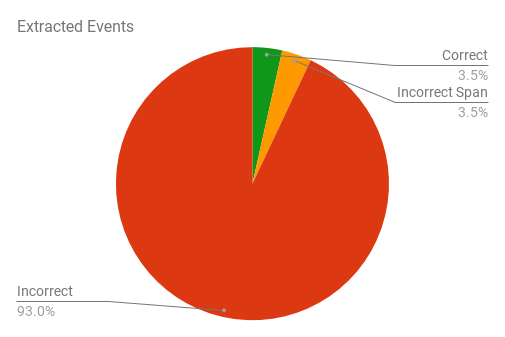
\includegraphics[width= 0.5\textwidth]{FrogEvents2}
  \caption{Result of the evaluation of the named events extracted with Frog.}
  \label{Frog events}
\end{figure}

\subsubsection{Analysis of Unnamed Event Extraction}\label{Analysis2}~\\
For the analysis of the unnamed event extraction we evaluate the sentences extracted with the 3-tier method. We also evaluate the event strings which we present in the metadata so that we can compare the performance. We consider the following three questions:
\begin{enumerate}
\item What percentage of the extracted sentences contained unnamed events?
\item If a sentence contains events, how many on average?
\item If a sentence did not contain an unnamed event, why?
\end{enumerate}

To answer the first two questions, the newly extracted sentences as well as the old events were manually evaluated by a single person. For each string the number of unnamed events were counted. Something was considered an event if 1. it was reported as something which has happened, might happen, or will happen at a later date, 2. the event is based on a verb or a set of verbs (i.e. unnamed events), and 3. the event has historic value (for example, we ignore regular weather events such as rain or wind coming from the west).

\textit{1. What percentage of the extracted sentences contained unnamed events?} Figure \ref{percentage eventful} shows the percentage of the extracted sentences that contained at least one historic unnamed event. We see that by searching for verbs, actors and places, we extract more sentences that are eventful. From the original events which were extracted by taking the first 100 characters only 8.4\% contained historic unnamed events. From the sentences that were extracted with the new 3-tier method 77.2\% was eventful. Thus the new method of extraction appears to be an improvement over the original events in the metadata of the bulletins.

\begin{figure}
  \centering
  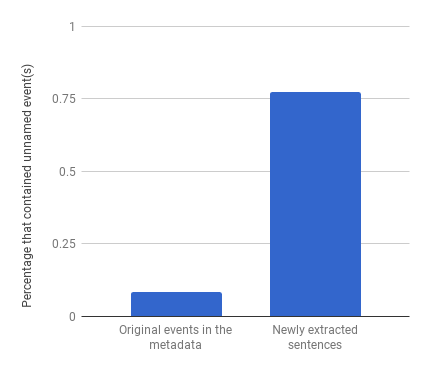
\includegraphics[width= 0.5\textwidth]{sentencesWithEvent2}
  \caption{A comparison between the old events in the metadata and the new events extracted with the 3-tier method. The figure compares the percentage of the sentences that were eventful.}
  \label{percentage eventful}
\end{figure}

\textit{2. If a sentence contains events, how many on average?}
We took all the extracted sentences and strings which were evaluated as eventful and looked at how many events they contained on average. The results are shown in figure \ref{events per sentence}. From the event strings in the metadata, we observe that the strings that were eventful contained exactly one event. From  the newly extracted sentences we see that the ones that were eventful contained more than one event on average. On the one hand, this means that these sentences likely contain more interesting and historical information. On the other hand, this also complicates a more fine grained event extraction. If a sentence contains some verbs, actors and places, we cannot say that those verbs, actors and place together form a single event. If for example a sentence contains two verbs, one actor and one place, it could be that the four entities are related together in a single event, or that the sentence contains two separate events, one described by a verb-actor relation and the other by a verb-place relation.

\begin{figure}
  \centering
  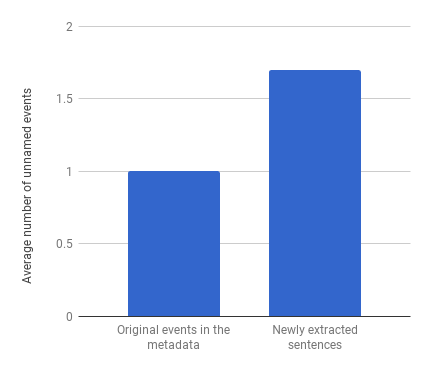
\includegraphics[width= 0.5\textwidth]{EventsPerSentence2}
  \caption{A comparison between the old events in the metadata and the new events extracted with the 3-tier method. The figure compares the average number of unnamed events found in eventful extracted sentences.}
  \label{events per sentence}
\end{figure}

\textit{3. If a sentence did not contain an unnamed event, why?}

We also examined the sentences that where extracted with the 3-tier method which did not contain any unnamed events. We identified the following reasons why these extracted sentences were uneventful:

\begin{itemize}
\item \textit{No new sentence was extracted.} As already mentioned and shown in table \ref{sentence extraction breakdown}, there were 23 bulletins in the dataset for which no new sentence was extracted with the 3-tier method. Reason for this was because TreeTagger recognized no verbs in the text of these bulletins. There are two situations in which this happened. Firstly, some bulletins simply had no verbs in the text. In the dataset this was mostly observed in sport segments which reported the result of sport matches or promotions and relegations in sports leagues. The second reason why no verb may be found in a text was due to errors produced by the OCR. As already mentioned in section \ref{data}, the OCR sometimes produces spelling errors in the extracted text by misidentifying characters in the documents. TreeTagger may not recognize any verbs when these errors happen in all the verbs in the text.
\item \textit{Words were incorrectly tagged as verbs.} Similarly to the previous point, errors produced by the OCR would sometimes cause TreeTagger to incorrectly identify words as verbs. For example, we witnessed a case where the OCR had extracted "derde" ("third") as "deerde" (past tense of "to harm"). The sentence was extracted because TreeTagger identified "deerde" as a verb, even though the sentence did not actually contain any verbs.
\item \textit{Incorrect sentence boundary detection.} Some of the extracted sentences were evaluated as being uneventful because the extracted sentence was not a full sentence. If a sentence contains a period character anywhere within the sentence and the period was not recognized as being part in an abbreviation, then the period would be assumed to be the end of the sentence, and the sentence would be cut short by the sentence boundary detection. These snippets of sentences might contain some verbs and NE's, but not all entities that are related to an event.

\item \textit{Incorrect Named Entities.} Lastly, we observed that some extracted sentences contained incorrect NE's. For instance, one of the extracted sentences which did not contain any unnamed events was \textit{"RADIO I. Eerste uitzending van 21 \^pril  Goedenavond Dames en Hoeren, Hier volgen Nieuwsberichten vanhot A. N. P.' Fublicatie, in welken vorm ook, is verboden."}. In this sentence \textit{"I. Eerste"} (I. First) and \textit{"Goedenavond Dames en Hoeren"} (Good evening Ladies and Gentlemen) had been classified as actors, and \textit{"Fublicatie"} (Publication) had been classified as a place. Eventhough actors, places and verbs had been identified, there is no actor-verb-place relationship present that represents a historic event.
\end{itemize}
We see with the first two observations that the quality of the OCR extraction negatively impacts the performance of the event extraction. Unfortunately we are unable to correct errors int the OCR text in the preprocessing step of the methodology using pattern-based search. The third and fourth observation will be addressed in the next step of the methodology.

%%%%%%%%%%%%%%%%%%%%%%%%%%%%%%%%%%%%%%%%%%%%%%%%%%%%%%%%%%%%%%%%%%%%%%%%%%%%

\subsection{Improving the Event Extraction}\label{improving}
In this step of the methodology we investigate ways to improve the event extraction through iterative steps. Since we have no control over the quality of the OCR text extraction or the performance of Frog for named event extraction, we will focus on improving the extraction of unnamed events. We will address possible improvements to the preprocessing step in section \ref{impr sbd}. In section \ref{impr NE} we explore the possibility of enriching the data with NER using Frog. Lastly, in section \ref{impr extraction} we examine assumptions we made in the unnamed event extract method. In each section we will formulate the issue, suggest and implement a possible solution, and analyze whether this resulted in improved event extraction.

\subsubsection{Improving Sentence Boundary Detection}\label{impr sbd}~\\
As noted in \ref{Analysis2}, errors in detection where sentences end occasionally result in extracting incomplete sentences. Period marks may appear in the middle of a sentence in four ways: in name initials, in abbreviations, in garbage strings, and in cases where the OCR misidentified characters as period marks. We already addressed the possibility of periods being part of name initials in the sentence boundary detection step in \ref{sbd} and included a pattern to detect initials as to not mark them as the end of a sentence. The option to improve garbage detection has already been addressed in \ref{garbage removal}. We observed that adding more pattern-based rules to increase the recall of garbage strings also increased the incorrect removal of strings that are not garbage. As mentioned previously, we also have no way to identify when the OCR software has misidentified a character. For example, The OCR may confuse a comma for a period, but we cannot detect this error because the period may appear as normal punctuation to a machine. 

This leaves us with periods appearing in abbreviations. We noticed that the most common abbreviations in the data were titles to address persons, such as \textit{prof.}, \textit{dr.} and \textit{mevr.} We hard-coded a list of titles that appear in the bulletins in the Java code that was written for the sentence boundary detection. Like the solution to initials, we check whether the characters directly before a period match any of the titles. 

We made this adjustment to the the sentence boundary detection, reran the unnamed event extraction and evaluated the extracted sentences that differed from the previously extracted ones. We found that this adjustment barely improved the event extraction, as the percentage of the extracted sentences that were eventful went up from 77.2\% to 79.2\%. But this was to be expected as originally only 7 sentences did not contain an event due to the sentence being incomplete, and of those 7 only 2 were cut short due to titles. 

\subsubsection{Using Frog for Named Entity Recognition}\label{impr NE}~\\
The extraction of unnamed events relies on finding relationships between verbs and NE's. But this can only be done successfully when the NE's are correctly extracted and typed. As noted in \ref{data} and \ref{Analysis2}, we see that the NE's in the metadata of the bulletins are not always correct.

We evaluated all the NE's in the data classified them into four categories: correctly extracted and typed, correctly typed but incorrect span, mistyped, and incorrect (not an NE). Since the evaluation was performed by a single person and human annotation is often ambiguous and open to multiple interpretations\cite{inel2017harnessing}\cite{aroyo2015truth}, we took a very liberal approach to the evaluation. We considered the span on an entity incorrect when it was very clearly too small (the extracted NE was incomplete) or too large (the extracted NE contained an actual NE of the correct type). For example, the inclusion or exclusion of articles did not affect whether the span was incorrect. The NE's in the metadata also do not include which instance of an entity was extracted when the entity appears multiple times in the text. For example, \textit{Duitschland} may appear multiple times in a text, and might act as a place in some context (\textit{"heeft HIMMLER het fransche katholieke orgaan" LA CROIX" in Duitschland verboden"}) and act as an actor in an other (\textit{"dat Duitschland besprekingen met Engeland had moeten voorstellen"}). When an NE appears multiple times in a text, we consider the type of the NE correct when it is correct for at least one of the instances.

The overall results of the evaluation of all NE's is shown in figure \ref{NE metadata evaluation}. Figures \ref{Actor metadata evaluation} and \ref{Place metadata evaluation} show the results of the actor and place entities only. Overall, we see that about a quarter of all the extracted NE's are incorrect or mistyped. Actors shows to have to larges percentage of usable extracted entities (those that were correct, or correct but with an incorrect span), while simultaneously also have the largest percentage of incorrectly extracted NE's (15.4\%). In figure \ref{Place metadata evaluation} we see that many of the mistyped NE's were typed as a place.

\begin{figure}
  \centering
  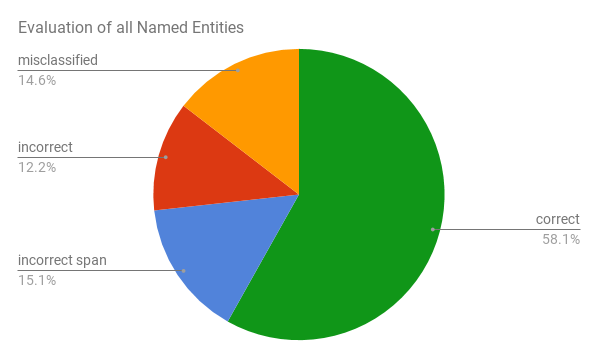
\includegraphics[width= 0.5\textwidth]{EvalNEsPaper}
  \caption{The evaluation of all Named Entities (actors, places, other concepts) in the metadata.}
  \label{NE metadata evaluation}
\end{figure}

\begin{figure}
  \centering
  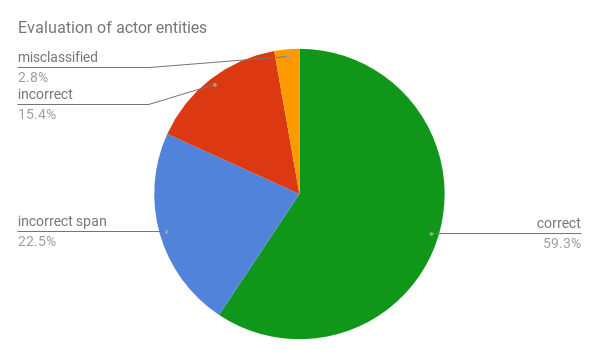
\includegraphics[width= 0.5\textwidth]{EvalActorsPaper}
  \caption{The evaluation of actor Named Entities in the metadata.}
  \label{Actor metadata evaluation}
\end{figure}

\begin{figure}
  \centering
  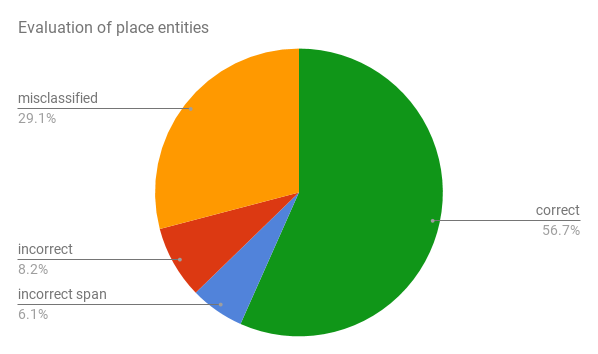
\includegraphics[width= 0.5\textwidth]{EvalPlacesPaper}
  \caption{The evaluation of place Named Entities in the metadata.}
  \label{Place metadata evaluation}
\end{figure}

The fact that a significant portion of the NE's of type actor and place are incorrect or incorrectly typed is problematic for the event extraction. If an extracted sentence contains for example a place, we cannot be absolutely sure that there is in fact a place mentioned in the sentence. It might actually be an actor, or worse, it might not be a relevant entity at all.
Another problem for the event extraction is, as mentioned earlier, the fact that an entity may appear multiple times in the text and we do not know whether an NE in the metadata refers to one instance or all the instances in the text. Furthermore, the fact that an entity may be classified as multiple types depending on the context is also problematic. If we look back at the previously mentioned example of \textit{Duitschland}, we see that when the metadata includes this entity twice, once as an actor and once as a place, then a sentence that includes \textit{Duitschland} may be extracted because the machine thinks that the sentence includes both an actor and a place.

To solve these issues we turn back to NER with Frog. As mentioned in \ref{named}, Frog is trained to extract NE's of type person, organization and location. Furthermore, Frog also specifies specifically which token in the text was labeled a NE. If a token appears multiple times in a text, we will know precisely to which instance the extracted NE refers. 

\begin{table}
  \begin{center}
    \begin{tabular}{l|r}
    NE type & Extracted\\
    \hline
    Person & 1,653\\
    Organisation & 1,382\\
    Location & 2,715\\
    Product & 270\\
    Miscellaneous & 1,696\\
    Event & 57\\
    \end{tabular}
  \end{center}
  \caption{The number of extracted Named Entities by Frog per type.}
  \label{Frog extraction breakdown}
\end{table}

We ran Frog on all the bulletins in the dataset and evaluated the extracted NE's of type person, organization and place.\footnote{Due to time constraints and the volume of extracted NE's, we evaluated the NE's extracted from 50 bulletins.} Since we are interested in whether NE's extracted by Frog are better suitable for our event extraction method, we make no distinction between NE's that are mistyped and extracted entities that aren't NE's (both are labeled as incorrect). Frog extracted a total of 7,773 NE's from 215 bulletins, table \ref{Frog extraction breakdown} shows the number of extracted NE's per type. 

The results of the evaluation is shown in figures \ref{Person Frog evaluation}, \ref{Org Frog evaluation} and \ref{Loc Frog evaluation}. Unfortunately we see that like the events, Frog also performs poorly for the extraction of the other entity types. Frog performed worse than the NER tool which was used to enrich the metadata of the bulletins. Hence we chose not to use the NE's extracted by Frog to perform the event extraction.

\begin{figure}[]
  \centering
  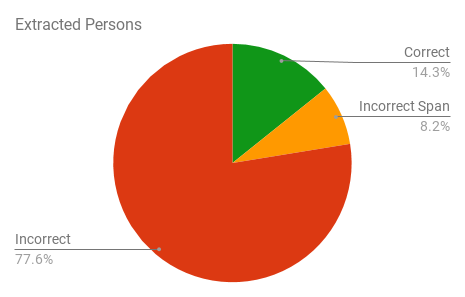
\includegraphics[width= 0.5\textwidth]{FrogPersons}
  \caption{The evaluation result of persons extracted by Frog.}
  \label{Person Frog evaluation}
\end{figure}

\begin{figure}[]
  \centering
  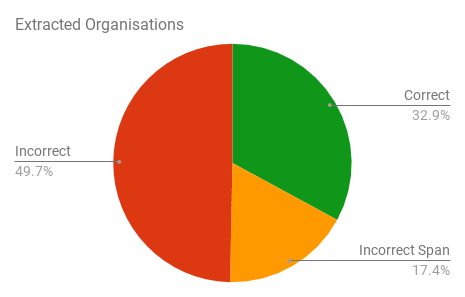
\includegraphics[width= 0.5\textwidth]{FrogOrganisations}
  \caption{The evaluation result of organisation extracted by Frog.}
  \label{Org Frog evaluation}
\end{figure}

\begin{figure}[]
  \centering
  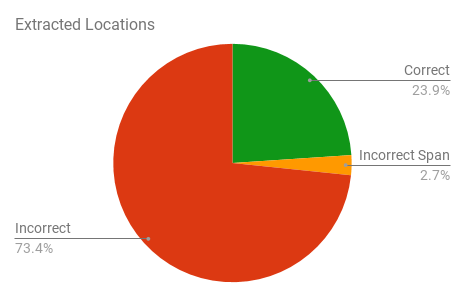
\includegraphics[width= 0.5\textwidth]{FrogLocations}
  \caption{The evaluation result of locations extracted by Frog.}
  \label{Loc Frog evaluation}
\end{figure}

\subsubsection{Assumptions of the Unnamed Event Extraction Approach}\label{impr extraction}~\\
In our method of unnamed event extraction we made two assumptions:
\begin{enumerate}
\item Sentences that contain a verb, an actor, and a place are more likely to contain unnamed events than sentences which do not have both an actor and place.
\item The main event or most important events are mentioned at the start of the text.
\end{enumerate}
We investigate these assumptions to see if these assumptions benefited the event extraction results. 

The 3-tier method for unnamed event extraction was based on assumption 1. We assumed that sentences that meet tier 1 are preferred over tier 2. However, in table \ref{sentence extraction breakdown} we saw that less than half of the bulletins in the dataset have a sentence that meets tier 1. This raises the question whether having tier 1 is beneficial. We tested the unnamed event extraction with a 2-tier method which is identical to the 3-tier method except that we omit tier 1. We evaluated the sentences extracted by the 2-tier system and compare them to the sentences extracted by the 3-tier method. Figure \ref{percentage eventful2} shows that fewer of the sentences extracted by the 2-tier method are eventful compared to the 3-tier method. Figure \ref{events per sentence2} shows that the sentences which were extracted by the 2-tier method that were eventful contain fewer events on average. We can thus conclude that sentences that meet the requirements of the first tier of the 3-tier method are in fact preferred for extraction. 

\begin{figure}
  \centering
  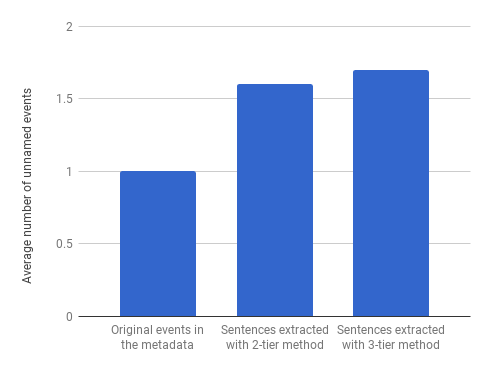
\includegraphics[width= 0.5\textwidth]{sentencesWithEvent}
  \caption{A comparison of the 2-tier method to the old events and 3-tier method. The figure compares the percentage of the sentences that were eventful.}
  \label{percentage eventful2}
\end{figure}

\begin{figure}
  \centering
  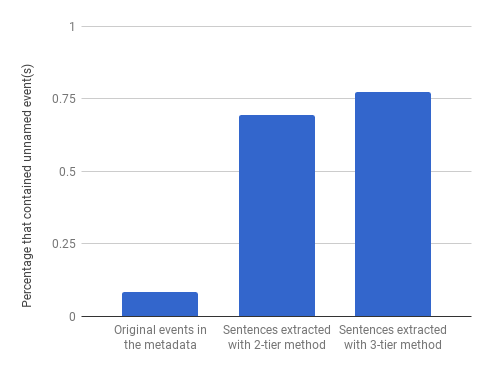
\includegraphics[width= 0.5\textwidth]{EventsPerSentence}
  \caption{A comparison of the 2-tier method to the old events and 3-tier method. The figure compares the average number of unnamed events found in eventful extracted sentences.}
  \label{events per sentence2}
\end{figure}

We extract the first sentence of a text that meets the requirements of one of the tiers because we assumed that main events are mentioned at the start of the text (assumption 2). However, when we look at the extracted events we see that many of the extracted sentence that have a verb, actor and place (tier 1) did not originate from the start of the text. We therefore look whether extracting from a specific part of the texts has an effect on the results.

Because the OCR did not preserve the formatting of the texts, we cannot split the texts by paragraphs. That is why we split all texts into three parts: a start, middle and end. For each text, the three parts are roughly equal length based on the number of sentences per part. We first look what the distribution of the types of sentences are. All sentences were labeled based on the 3 tiers of the extraction method: meets tier 1, meets tier 2, meets tier 3, and sentences that have no verbs. We counted the sentences per text part, the result is shown in figure \ref{sentence dist}. We see that there are more sentences without verbs near the start of the text. This corresponds with the observation that many of the bulletins start with header information, which mostly consists of short sentences without verbs. However, we see that the distribution of sentences that meet any of the 3 tiers does not vary much between the parts of the texts.

\begin{figure}
  \centering
  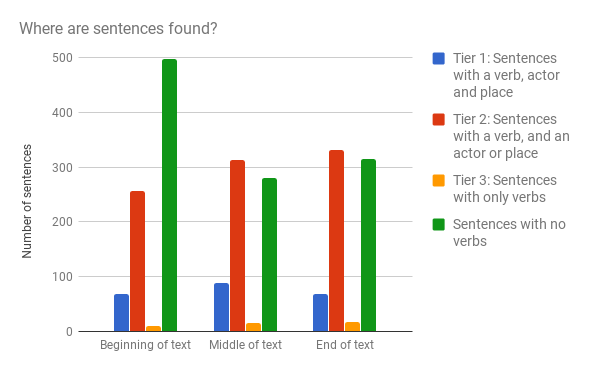
\includegraphics[width= 0.5\textwidth]{WhereAreSentencesFound}
  \caption{A comparison of the 2-tier method to the old events and 3-tier method. The figure compares the average number of unnamed events found in eventful extracted sentences.}
  \label{sentence dist}
\end{figure}

We examine if extracting a sentence from a specific part of the text affects the results. For each bulletin, we extracted a new sentence using the 3-tier from each of the three parts of the texts. The extracted sentences were evaluated for the number of unnamed historical events\footnote{Due to time constraints we evaluated sentences extracted for 130 bulletins.} and compared to the sentence we extracted from the full texts. Figure \ref{sentence dist extraction1} and \ref{sentence dist extraction2} show the results of this comparison. We see that by limiting the sentence extraction to a specific part of the text we are less likely to extract an eventful sentence (fig.\ref{sentence dist extraction1}). The sentence extracted from the start or middle of the text that are eventful contain slightly fewer events on average, and sentences that are extracted from the end part of the text that are eventful have slightly more events on average, but the difference is very minimal (fig.\ref{sentence dist extraction2}). We thus conclude that limiting the extraction to a specific part of the text results in slightly worse event extraction. We suspect that the reason for this is that by limiting the extraction to a specific part of the text, the extractor might be forced to extract a sentence that matches a lower tier. If a text is only contains one sentence that has a verb, an actor and a place, then by extracting from a specific part of the text we will not extract this sentence if it is not in the specified part.

\begin{figure}
  \centering
  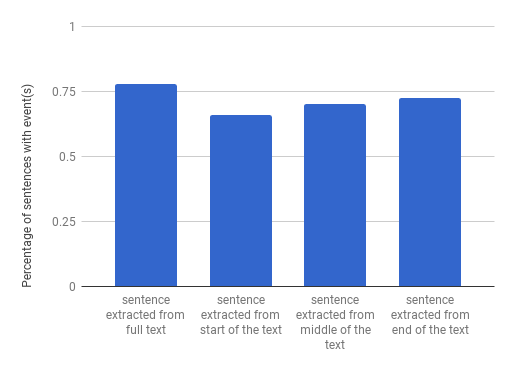
\includegraphics[width= 0.5\textwidth]{percentageEventfulDist2}
  \caption{A comparison of sentences extracted from a specific part of the texts. The figure compares the percentage of the sentences that were eventful.}
  \label{sentence dist extraction1}
\end{figure}

\begin{figure}
  \centering
  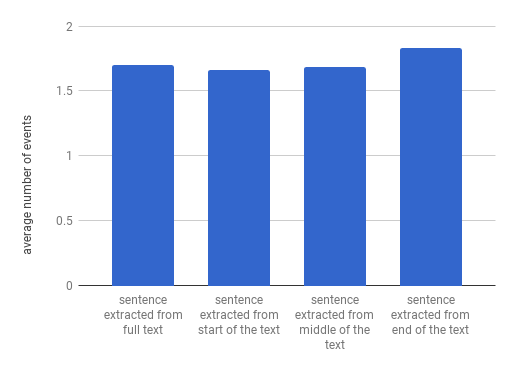
\includegraphics[width= 0.5\textwidth]{averageNrOfEventsDist2}
  \caption{A comparison of sentences extracted from a specific part of the texts. The figure compares the average number of unnamed events found in eventful extracted sentences.}
  \label{sentence dist extraction2}
\end{figure}

%%%%%%%%%%%%%%%%%%%%%%%%%%%%%%%%%%%%%%%%%%%%%%%%%%%%%%%%%%%%%%%%%%%%%%%%%%%%%%%%

\section{Results}
With the proposed methodology we successfully improved upon the old event extraction method. By extracting sentences using the 3-tier method we extracted an eventful sentence for 79.2\% of the bulletins in the data. The extraction of named events was unfortunately unsuccessful. Errors in OCR often have a detrimental effect on the performance of NER\cite{alex2014estimating} and Frog was no exception. Because Frog performed poorly at extracting named events (precision of 7,0\%) it was decided to not enrich the metadata of the bulletins with the events extracted by Frog as they would likely cause false links to be created in the linked data structure. We did replace the old events in the metadata of the radio news bulletins with the sentences extracted with the unnamed event extraction method.

[Results of the final bit of analysis to be written here]
%%%%%%%%%%%%%%%%%%%%%%%%%%%%%%%%%%%%%%%%%%%%%%%%%%%%%%%%%%%%%%%%%%%%%%%%%%%%%%%%

\section{Discussion}


\section{Conclusion}


%%%%%%%%%%%%%%%%%%%%%%%%%%%%%%%%%%%%%%%%%%%%%%%%%%%%%%%%%%%%%%%%%%%%%%%%%%%%%%%%

\section{Future Work}

\bibliographystyle{unsrt}
%\bibliographystyle{ACM-Reference-Format}
\bibliography{bibliography} 

\onecolumn
\section{Appendix}
\appendix
\begin{figure}[H]
  \centering
  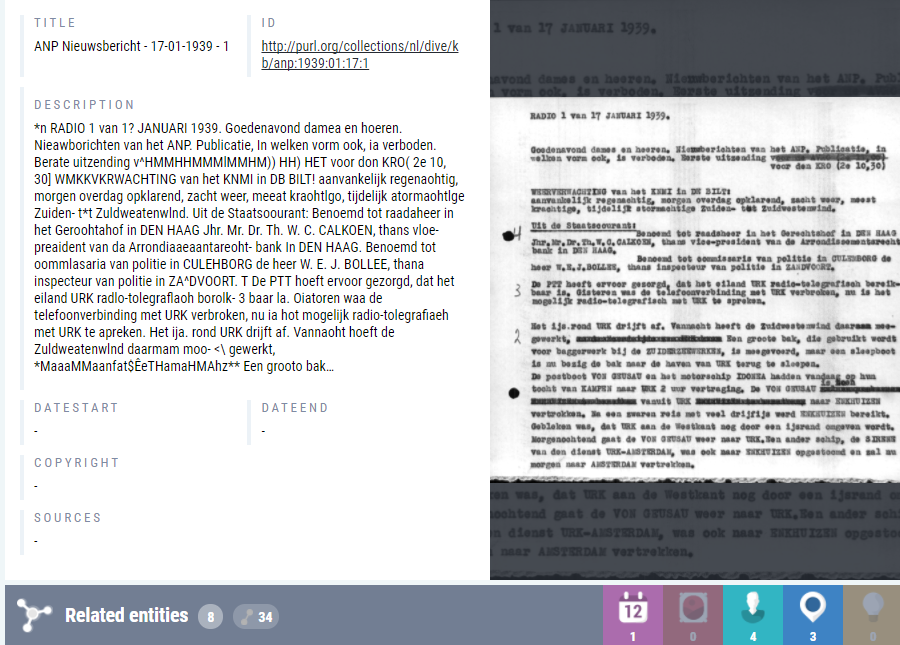
\includegraphics[width= \textwidth]{bulletin2}
  \caption{An example of an ANP radio news bulletins in the DIVE+ demonstrator. }
  \label{bulletin}
\end{figure}

\end{document}